\capitulo{4}{Técnicas y herramientas}

Este capítulo presenta las metodologías de trabajo, los entornos de desarrollo y el conjunto de herramientas utilizadas para construir el proyecto. Para cada elemento del sistema, se describen sus funciones esenciales, la justificación de su elección frente a otras alternativas del mercado y cómo se integran dentro del flujo continuo de datos del pipeline.

\section{Metodología de trabajo}
La organización y el desarrollo del proyecto se han estructurado siguiendo un enfoque ágil basado en Sprints o ciclos de trabajo de aproximadamente dos semanas de duración. Esta metodología consiste en fragmentar el objetivo general del desarrollo en pequeñas tareas más manejables que se puedan planificar, programar y probar en plazos de tiempo reducidos. 

Para gestionar este flujo de trabajo de forma visual se ha empleado el sistema Kanban. Las tareas se representan en tarjetas individuales que se mueven a lo largo de un tablero dividido en columnas según su estado actual: pendientes de inicio, en proceso de desarrollo, en fase de pruebas o finalizadas correctamente. Además, para medir la carga de trabajo de cada Sprint, se han asignado puntos de esfuerzo abstractos a cada tarea. Esto permite flexibilizar el calendario de trabajo y adaptar el desarrollo al ritmo real del proyecto, priorizando siempre la estabilidad de los componentes críticos antes de avanzar.

\section{Sistema de control de versiones (Git)}
Git es un sistema de control de versiones que funciona a nivel local en el ordenador de desarrollo. Su objetivo principal en este proyecto ha sido realizar un seguimiento histórico de todos los avances y cambios realizados en el código fuente del software a lo largo del proyecto.

A diferencia de desarrollos en equipo donde se gestionan múltiples ramas paralelas, en este trabajo se ha utilizado Git de una forma lineal y directa sobre la línea principal de código. Su utilidad real ha sido registrar de manera ordenada cada modificación en los scripts de Python y en los archivos de configuración dentro del equipo local. Esto permite disponer de un historial seguro de versiones anteriores al que poder recurrir de inmediato si un cambio nuevo falla, sirviendo además como la herramienta clave para empaquetar y enviar todo el trabajo hacia el repositorio remoto de forma fácil, cómoda y rápida.

\begin{figure}[h]
    \centering
    
\includegraphics[height=1.25cm]{img/logo_git.png}
    \caption{Logotipo del sistema de control de versiones Git.}
    \label{fig:logo_git}
\end{figure}

\section{Plataforma central de desarrollo y automatización (GitHub)}
GitHub constituye el nodo central sobre el que se apoya toda la infraestructura, la gestión de tareas y la automatización del proyecto, unificando diferentes procesos en un único entorno:

\begin{figure}[h]
    \centering
    
\includegraphics[height=2cm]{img/logo_github.png}
    \caption{Logotipo de la plataforma GitHub.}
    \label{fig:logo_github}
\end{figure}

\subsection{Gestión de tareas y repositorio}
A través de las extensiones de GitHub Projects y Zenhub se implementó el tablero Kanban del proyecto, permitiendo asociar directamente las tarjetas de tareas con las líneas de código modificadas. Asimismo, la plataforma funciona como el repositorio remoto del proyecto, asegurando el almacenamiento seguro de los scripts y el control de los cambios síncronos combinados con Git local.

\begin{figure}[h]
    \centering
    
\includegraphics[height=2cm]{img/logo_zenhub.png}
    \caption{Logotipo de la plataforma de gestión Zenhub.}
    \label{fig:logo_zenhub}
\end{figure}

\subsection{Automatización del pipeline (GitHub Actions)}
Para lograr que el sistema funcione de forma autónoma sin depender de un ordenador físico encendido, se evaluó el uso de Google Cloud Functions. Sin embargo, este servicio se descartó debido a su límite estricto de ejecución de 9 minutos por función y a que Google cobra por la memoria RAM consumida mientras el proceso está activo. 

En su lugar se eligió GitHub Actions, configurado mediante un  workflow que permite programar la ejecución de forma cíclica a través de un cron personalizable, realizando las ejecuciones periódicas del scraper de forma completamente automática \cite{github_actions_docs}. Esta elección se justifica porque ofrece hasta 2.000 minutos mensuales de computación gratuita para repositorios públicos, permite tiempos de ejecución continuos de hasta 6 horas y regala una máquina virtual con 7 GB de memoria RAM, siendo una opción claramente mejor de automatización que Google Cloud Functions.

\begin{figure}[h]
    \centering
    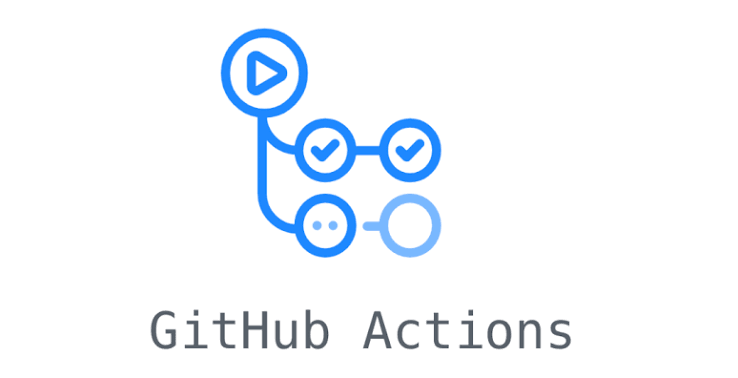
\includegraphics[height=3cm]{img/logo_github_actions.png}
    \caption{Logotipo del motor de automatización GitHub Actions.}
    \label{fig:logo_github_actions}
\end{figure}

\subsection{Seguridad y credenciales (GitHub Secrets)}
Debido a que el script automático en la nube debe conectarse de forma autónoma con Google Cloud para escribir datos en la base de datos, se utiliza la funcionalidad de GitHub Secrets. Esta herramienta cifra la contraseña en los servidores de GitHub con el nombre \texttt{GCP\_SA\_KEY} y solo se la entrega de forma segura al motor de Actions en el momento exacto de la ejecución del programa.

Debido a que el script automático en la nube debe ejecutarse solo y conectarse de forma autónoma tanto con el servicio de extracción como con Google Cloud, el sistema requería el uso de claves de acceso seguras utilizando la funcionalidad de GitHub Secrets. 

Esta herramienta cifra las credenciales en los servidores de GitHub y solo se las entrega de forma segura al motor de Actions en el momento exacto en el que arranca el programa. En este proyecto se han configurado dos secretos esenciales:
\begin{itemize}
    \item \textbf{Token de Apify:} La clave privada necesaria para autenticar el script de Python con la plataforma de extracción.
    \item \textbf{Llave de Google Cloud (\texttt{GCP\_SA\_KEY}):} El archivo JSON de la cuenta de servicio que da permiso al pipeline para entrar en Google Cloud y escribir de forma directa los nuevos datos dentro de la tabla de BigQuery.
\end{itemize}

\section{Entorno de desarrollo local (Visual Studio Code)}
La escritura, pruebas locales y edición de todos los componentes se han realizado sobre el entorno de desarrollo integrado Visual Studio Code (VSCode). Se eligió esta herramienta frente a otras alternativas pesadas por su ligereza en memoria y por su capacidad para unificar en una sola interfaz la edición de los archivos de código, la visualización de la estructura de las carpetas, el uso de extensiones de depuración y la terminal de comandos del sistema operativo local.

\begin{figure}[h]
    \centering
    
\includegraphics[height=2cm]{img/logo_vscode.png}
    \caption{Logotipo del entorno de desarrollo Visual Studio Code.}
    \label{fig:logo_vscode}
\end{figure}

\section{Herramienta de extracción (Apify)}
La elección del mecanismo para descargar la información de Google Maps fue uno de los debates técnicos más importantes del proyecto. Se evaluaron cuatro alternativas principales antes de tomar la decisión definitiva:
\begin{itemize}
    \item \textbf{API oficial de Google Places:} Se descartó por completo debido a tres problemas insalvables: limita la descarga a un máximo de 5 reseñas por sitio, tiene un coste económico alto por cada petición y sus términos legales prohíben almacenar sus datos en una base de datos propia por más de 30 días.
    \item \textbf{Script propio con Playwright:} Planteado originalmente como el Plan A. El código utilizaba selectores basados en roles de accesibilidad para esquivar los cambios continuos que hace Google en el diseño de su interfaz. Sin embargo, se descartó por completo debido a la imposibilidad técnica de crear un capturador propio capaz de superar las estrictas medidas de seguridad de una empresa como Google, que detecta y bloquea de inmediato las extracciones masivas de datos mediante sistemas antibot y controles de dirección IP.
    \item \textbf{Servicios externos de pago (Outscraper, SerpApi o ValueSerp):} Estas APIs entregan la información de forma directa, pero funcionan como una "caja negra" sin control sobre el proceso y suelen generar fallos al exportar a formatos tradicionales como CSV debido a que las comas de los textos largos rompen las tablas.
    \item \textbf{Plataforma Apify (Opción elegida):} Se seleccionó como la herramienta de extracción central utilizando el componente desarrollado por \textit{Compass} \cite{apify_scraper_compass} , que es el más completo y económico para cuentas gratuitas.
    
    \item \textbf{Plataforma Apify (Opción elegida):} Se seleccionó como la herramienta de extracción central utilizando los componentes desarrollados por \textit{Compass}, el scraper de POIs \cite{apify_scraper_compass} y el scraper de reseñas \cite{apify_reviews_scraper_compass}.
\end{itemize}

La elección de Apify se justifica porque lanza un navegador automático en un servidor propio que entra en la web, imita las acciones de una persona haciendo desplazamientos hacia abajo para forzar la carga de todas las reseñas de la pantalla y las lee directamente. Al trabajar de forma nativa en formato JSON, se garantiza la integridad de los textos sin peligro de que los caracteres especiales rompan las columnas de la base de datos. Además, ofrece una librería oficial para Python y funciona mediante un sistema cerrado de créditos que detiene el script si el saldo se agota, aportando una seguridad que evita facturas imprevistas.

\begin{figure}[h]
    \centering
    
\includegraphics[height=2cm]{img/logo_apify.png}
    \caption{Logotipo de la plataforma de extracción web Apify.}
    \label{fig:logo_apify}
\end{figure}

\section{Infraestructura de almacenamiento (Google BigQuery)}
Para guardar toda la información, se descartó el uso de bases de datos relacionales tradicionales locales (como MySQL en Laragon) porque obligaban a mantener un servidor físico encendido y requerían exportar archivos intermedios de forma manual para actualizar los gráficos. En su lugar, se eligió Google BigQuery.

BigQuery es un almacén de datos analítico en la nube, totalmente gestionado y optimizado para ejecutar consultas complejas sobre grandes volúmenes de información. Su elección dentro de la arquitectura del proyecto se justifica por los siguientes criterios técnicos y operativos:
\begin{itemize}
    \item \textbf{Accesibilidad y automatización en la nube:} Al ser un servicio basado en la nube, elimina por completo la necesidad de mantener un servidor físico local encendido de forma continua. Esto permite que los scripts automáticos guarden la información directamente en internet, logrando que todo el sistema de información funcione de manera autónoma en todo momento sin depender de un ordenador personal.
    \item \textbf{Conexión nativa con el cuadro de mando:} Al pertenecer al mismo ecosistema de herramientas de Google que Looker Studio, la comunicación entre la base de datos y la plataforma de visualización es directa y transparente. Esto elimina la necesidad de descargar y subir manualmente archivos intermedios en formato CSV desde el entorno local, permitiendo que el Boletín de Turismo consulte la base de datos en tiempo real y permanezca actualizado de forma automática.
    \item \textbf{Viabilidad económica (Modalidad Sandbox):} BigQuery ofrece una capa gratuita permanente que permite almacenar hasta 10 GB de datos y procesar hasta 1 TB de consultas mensuales sin coste. Esta capacidad es más que suficiente para gestionar el histórico de puntos de interés y reseñas analizadas en el proyecto a coste cero.
\end{itemize}

\begin{figure}[h]
    \centering
    
\includegraphics[height=2.5cm]{img/logo_bigquery.jpg}
    \caption{Logotipo del almacén de datos Google BigQuery.}
    \label{fig:logo_bigquery}
\end{figure}
\section{Contenedorización (Docker)}
Para asegurar la portabilidad del proyecto se ha utilizado Docker mediante la configuración de un archivo \texttt{Dockerfile} y un fichero de dependencias \texttt{requirements.txt}. 

La utilización de Docker se justifica porque crea un entorno estándar aislado y reproducible. Si el entorno de Python local del ordenador de desarrollo se actualiza o rompe sus librerías, el sistema sigue funcionando correctamente dentro del contenedor independiente. El \texttt{Dockerfile} define el entorno estándar del proyecto, asegurando que el scraper funcione en cualquier sistema.

\begin{figure}[h]
    \centering
    
\includegraphics[height=2.4cm]{img/logo_docker.png}
    \caption{Logotipo de la plataforma de contenedores Docker.}
    \label{fig:logo_docker}
\end{figure}

\section{Lenguajes de programación}
La construcción, automatización y documentación del proyecto ha requerido la intervención de diferentes lenguajes:
\begin{itemize}
    \item \textbf{Python 3.13:} El lenguaje de programación principal utilizado para escribir todos los scripts que componen la lógica del pipeline.
    \item \textbf{SQL (Google Standard SQL):} Es el lenguaje de consultas utilizado en BigQuery. Se ha usado constantemente para crear las tablas, insertar valores manuales de prueba, hacer consultas \texttt{SELECT} para comprobar los datos y, dentro del propio código de Python, para lanzar las consultas de subida de los nuevos datos extraídos.
    \item \textbf{LaTeX:} El lenguaje utilizado para escribir, estructurar y dar formato profesional a la memoria y los anexos de la documentación.
    \item \textbf{YAML:} El formato de datos utilizado para redactar el workflow de GitHub Actions, especificando los pasos y los horarios del servidor automático.
    \item \textbf{Markdown:} Lenguaje empleado para redactar los archivos (\texttt{README}) informativos del repositorio del proyecto.
\end{itemize}

\section{Bibliotecas de procesamiento de datos y conectores}
Para realizar las tareas de extracción, limpieza, traducción y análisis dentro del código de Python, se han utilizado las siguientes librerías:

\begin{itemize}
    \item \textbf{\texttt{apify-client}:} Es la librería oficial de Apify para Python. Se encarga de inicializar el cliente operativo mediante el token, lanzar los actores de Google Maps en la nube y descargar los resultados de puntos de interés y reseñas de forma incremental en formato JSON \cite{pypi_apify_client}.
    \item \textbf{\texttt{google-cloud-bigquery}:} Conector oficial de Google Cloud Platform. Permite que el script \ruta{bigquery\_loader.py} se autentique de forma segura, cree las tablas temporales de carga y ejecute de forma directa las sentencias SQL y las fusiones mediante \texttt{MERGE} \cite{pypi_bigquery}.
    \item \textbf{\texttt{pysentimiento}:} Es la librería encargada del análisis de sentimiento de los textos de las reseñas. El modelo calcula las probabilidades de que una reseña sea positiva, neutra o negativa, permitiendo al script realizar el cálculo matemático de restar la probabilidad negativa a la positiva para obtener una nota continua en el rango exacto de $[-1, 1]$ \cite{pypi_pysentimiento}.
    \item \textbf{\texttt{langdetect}:} Biblioteca utilizada dentro del módulo de transformación para identificar automáticamente el idioma original en el que el turista escribió la reseña, sirviendo de filtro previo antes de decidir si el texto necesita traducción.
    \item \textbf{\texttt{deep-translator}:} Herramienta utilizada para conectar con el motor de Google Translate de forma gratuita. Traduce automáticamente al idioma pedido los textos de las opiniones extranjeras detectadas por \texttt{langdetect}, permitiendo almacenar en la base de datos tanto la versión original como la traducida \cite{pypi_deep_translator}.
    \item \textbf{\texttt{gender-guesser}:} Librería de detección de género. Analiza el primer nombre del autor de la reseña y lo clasifica automáticamente como "Masculino" o "Femenino". En caso de nombres ambiguos, perfiles de empresas o cuentas privadas, permite inyectar el valor "Desconocido" por defecto configurado en el sistema.
\end{itemize}

\section{Herramienta de cuadro de mando y visualización (Looker Studio)}
La fase de explotación final de los datos se ha desarrollado sobre la plataforma Looker Studio. Aunque se estudió el uso de herramientas líderes del mercado como Power BI, su elección final vino impuesta por una restricción técnica del servidor del propio Observatorio de Turismo, que exigía para su servidor la utilización de Looker Studio en su lugar.

De este modo, Looker Studio se justifica como la única solución viable por los siguientes motivos:
\begin{itemize}
    \item \textbf{Gratuidad y acceso web:} Es una herramienta totalmente gratuita basada en la nube que permite diseñar gráficos interactivos sin costes de licencias.
    \item \textbf{Conexión nativa con BigQuery:} Al pertenecer ambas herramientas al ecosistema de Google, la sincronización de las tablas de datos es directa y automática, lo que permite que los gráficos se actualicen solos en cuanto el pipeline añade nuevos registros, sin necesidad de abrir el portátil ni ejecutar nada.
    \item \textbf{Facilidad de integración:} Permite generar códigos de incrustación seguros para insertar el cuadro de mando de manera transparente dentro del portal web de la institución.
\end{itemize}

\begin{figure}[h]
    \centering
    
\includegraphics[height=2.5cm]{img/logo_looker.jpg}
    \caption{Logotipo de la herramienta de visualización Looker Studio.}
    \label{fig:logo_looker}
\end{figure}

\section{Herramientas de diseño gráfico y diagramas (Draw.io)}
Para la fase de diseño de la arquitectura del sistema y la creación de los diagramas técnicos de la memoria, se ha utilizado la herramienta web Draw.io. Esta aplicación permite diseñar de forma visual y personalizada la estructura de los componentes informáticos mediante plantillas estándar.

\begin{figure}[h]
    \centering
    
\includegraphics[height=2.5cm]{img/logo_drawio.png}
    \caption{Logotipo de la herramienta de diagramas Draw.io.}
    \label{fig:logo_drawio}
\end{figure}

\section{Herramientas de asistencia (Gemini)}
Se ha empleado la herramienta de inteligencia artificial Gemini como recurso de apoyo consultivo durante el desarrollo del proyecto. Su uso ha consistido en resolver dudas técnicas de programación y a agilizar el diseño del pipeline.

Entre los casos concretos de uso se incluye la corrección de errores de la terminal al ejecutar el sistema, el soporte para estructurar algunas consultas SQL dentro de BigQuery, la resolución de dudas teóricas sobre el proyecto y la ayuda con el formato de las etiquetas de \LaTeX{} para la maquetación de esta memoria.

\begin{figure}[h]
    \centering
    
\includegraphics[height=2.5cm]{img/logo_gemini.jpg}
    \caption{Logotipo del asistente técnico Gemini.}
    \label{fig:logo_gemini}
\end{figure}